\documentclass[aspectratio=169, 12pt]{beamer}

% --- Balíčky pro češtinu, obrázky a formátování ---
\usepackage{inputenc}
\usepackage[czech]{babel}
\usepackage{graphicx}
\usepackage{booktabs}
\usepackage{caption}

% --- Vzhled prezentace ---
\usetheme{Madrid}
\usecolortheme{beaver} 

% Odstranění navigačních symbolů
% \setbeamertemplate{navigation symbols}{}

% --- Údaje o práci ---
\title[GoodAccess CLI]{GoodAccess CLI klient pro Linux}
\subtitle{Bakalářská práce}
\author{Valdemar Pospíšil}
\institute[UJEP]{
  Přírodovědecká fakulta UJEP \\
  Studijní program: Aplikovaná informatika
}
\date{} % Datum prázdné

% Definice vedoucího
\newcommand{\supervisor}{Ing. Jiří Hromádka}

% --- Loga na titulní straně (dole) ---
\titlegraphic{
   % Pokud nemáš obrázky, zakomentuj tyto řádky pomocí %
   
\includegraphics[height=2.5cm]{images/ujep_logo.jpg}
   \hspace{8cm} 
   
\includegraphics[height=2.5cm]{images/goodaccess.jpg}
}

\begin{document}

% =========================================================================
% SLIDE 1: Titulní strana
% =========================================================================
\begin{frame}
    \titlepage
    \vspace{-2.5cm}
    \begin{center}
        \small Vedoucí práce: \supervisor
    \end{center}
\end{frame}

% =========================================================================
% SLIDE 2: Motivace a Cíle
% =========================================================================
\begin{frame}{Motivace a cíle práce}
    
        \centering
        \textbf{Motivace}

        \vspace{0.5cm}
    
        % První řádek
        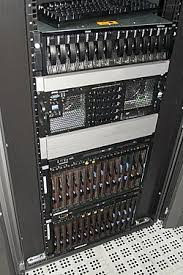
\includegraphics[height=2cm]{images/server.jpg} \hspace{1cm}
        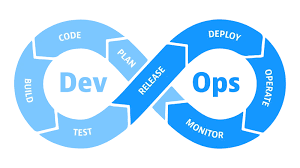
\includegraphics[height=2cm]{images/devops.png} \hspace{1cm}
        
\includegraphics[height=2cm]{images/terminal.png}
        
        %\begin{itemize}
        %    \item \textbf{Serverové prostředí:} Nutnost správy VPN na Linux serverech bez GUI (Headless mode).
         %   \item \textbf{DevOps a Automatizace:} Možnost skriptování připojení v CI/CD pipelinách.
         %   \item \textbf{Efektivita:} Rychlá správa připojení z terminálu.
       % \end{itemize}

        \vspace{0.4cm}
        
        \textbf{Cíle práce}
        \begin{itemize}
            \item \textbf{Backend (.NET):} Implementace modulu \texttt{CLIService} pro logiku autentizace a řízení tunelu.
            \item \textbf{Frontend (Go):} Vývoj nativního CLI klienta.
            \item \textbf{Funkcionalita:} Přihlášení, správa VPN, monitoring stavu.
            \item \textbf{Distribuce:} Tvorba instalačních balíčků (.deb/.rpm).
        \end{itemize}

      
        % Pokud nemáš obrázek usecase.png, zakomentuj řádek níže
       % \includegraphics[width=\textwidth]{usecase.png}
\end{frame}

% =========================================================================
% SLIDE 3: Současný stav poznání
% =========================================================================
\begin{frame}{Současný stav poznání}
    \textbf{Moderní "Command-Line First" přístup}
    \begin{itemize}
        \item Odklon od monolitických aplikací k jednoúčelovým utilitám.
        \item Důraz na strojově čitelný výstup (JSON) umožňující integraci s dalšími nástroji (Ansible, Terraform).
    \end{itemize}
    
    \vspace{0.5cm}
    
    \textbf{Meziprocesní komunikace (IPC) v Linuxu}
    \begin{itemize}
        \item Využití \textbf{Unix Domain Sockets} jako standardu pro bezpečnou lokální komunikaci.
        \item Výhody: Vyšší výkon a možnost řízení přístupových práv přes souborový systém.
    \end{itemize}
\end{frame}

% =========================================================================
% SLIDE 4: Teoretická východiska
% =========================================================================
\begin{frame}{Teoretická východiska}
    \textbf{Clean Architecture}
    \begin{itemize}
        \item Oddělení prezentační vrstvy (Go CLI) od aplikační logiky (.NET Service).
        \item Nezávislost na konkrétním uživatelském rozhraní (CLI/GUI).
    \end{itemize}

    \vspace{0.3cm}

    \textbf{Metodika vývoje (XP)}
    \begin{itemize}
        \item \textbf{Agilní principy:} Flexibilní reakce na změny a průběžná integrace.
        \item \textbf{Iterační vývoj:} Práce v krátkých cyklech (sprinty).
        \item \textbf{Test-Driven Development (TDD):} Cyklus Red-Green-Refactor pro zajištění stability kódu.
        \item \textbf{Behavior Driven Development (BDD):} Definice akceptačních kritérií pomocí Gherkin scénářů.
    \end{itemize}
\end{frame}

% =========================================================================
% SLIDE 5: Metodika řešení
% =========================================================================
%\begin{frame}{Metodika řešení}
%    \begin{enumerate}
%        \item \textbf{Analýza a návrh:}
%        \begin{itemize}
%            \item Definice komunikačního protokolu (IPC kontrakt).
%            \item Identifikace klíčových scénářů (Login, Connect, Status).
%        \end{itemize}
        
%        \item \textbf{Implementace:}
%        \begin{itemize}
%            \item Backend: Rozšíření \texttt{GoodAccessService} o modul pro CLI.
%            \item Frontend: Implementace příkazů v Go (Cobra framework).
%        \end{itemize}
        
%        \item \textbf{Integrace a testování:}
%        \begin{itemize}
%            \item Propojení frontendu a backendu přes sokety.
%            \item Řešení souběžných stavů (konflikty mezi GUI a CLI).
%        \end{itemize}
%    \end{enumerate}
%\end{frame}

% =========================================================================
% SLIDE 6: Praktická část - Implementace
% =========================================================================
\begin{frame}{Praktická část: Použité technologie}
    \centering
    \vspace{0.5cm}
    
    % První řádek
    
\includegraphics[height=1.8cm]{images/go.png} \hspace{1cm}
    
\includegraphics[height=1.8cm]{images/csharp.png} \hspace{1cm}
    
\includegraphics[height=1.8cm]{images/dotnet.png}
    
    \vspace{1cm} % Mezera mezi řádky
    
    % Druhý řádek
    
\includegraphics[height=1.5cm]{images/linux.jpg} \hspace{1cm}
    
\includegraphics[height=1.5cm]{images/cobra.png} \hspace{1cm}
    
\includegraphics[height=1.5cm]{images/bubbletea.jpg}
    
    \vspace{1cm} % Mezera mezi řádky

    % Třetí řádek
    
\includegraphics[height=1.5cm]{images/gitlab.png} \hspace{1cm}
    
\includegraphics[height=1.5cm]{images/slack.png}

\end{frame}

\begin{frame}{Praktická část: Návrh komunikace (IPC)}
    \centering
    % Diagram zabere většinu obrazovky, keepaspectratio zachová poměr stran
    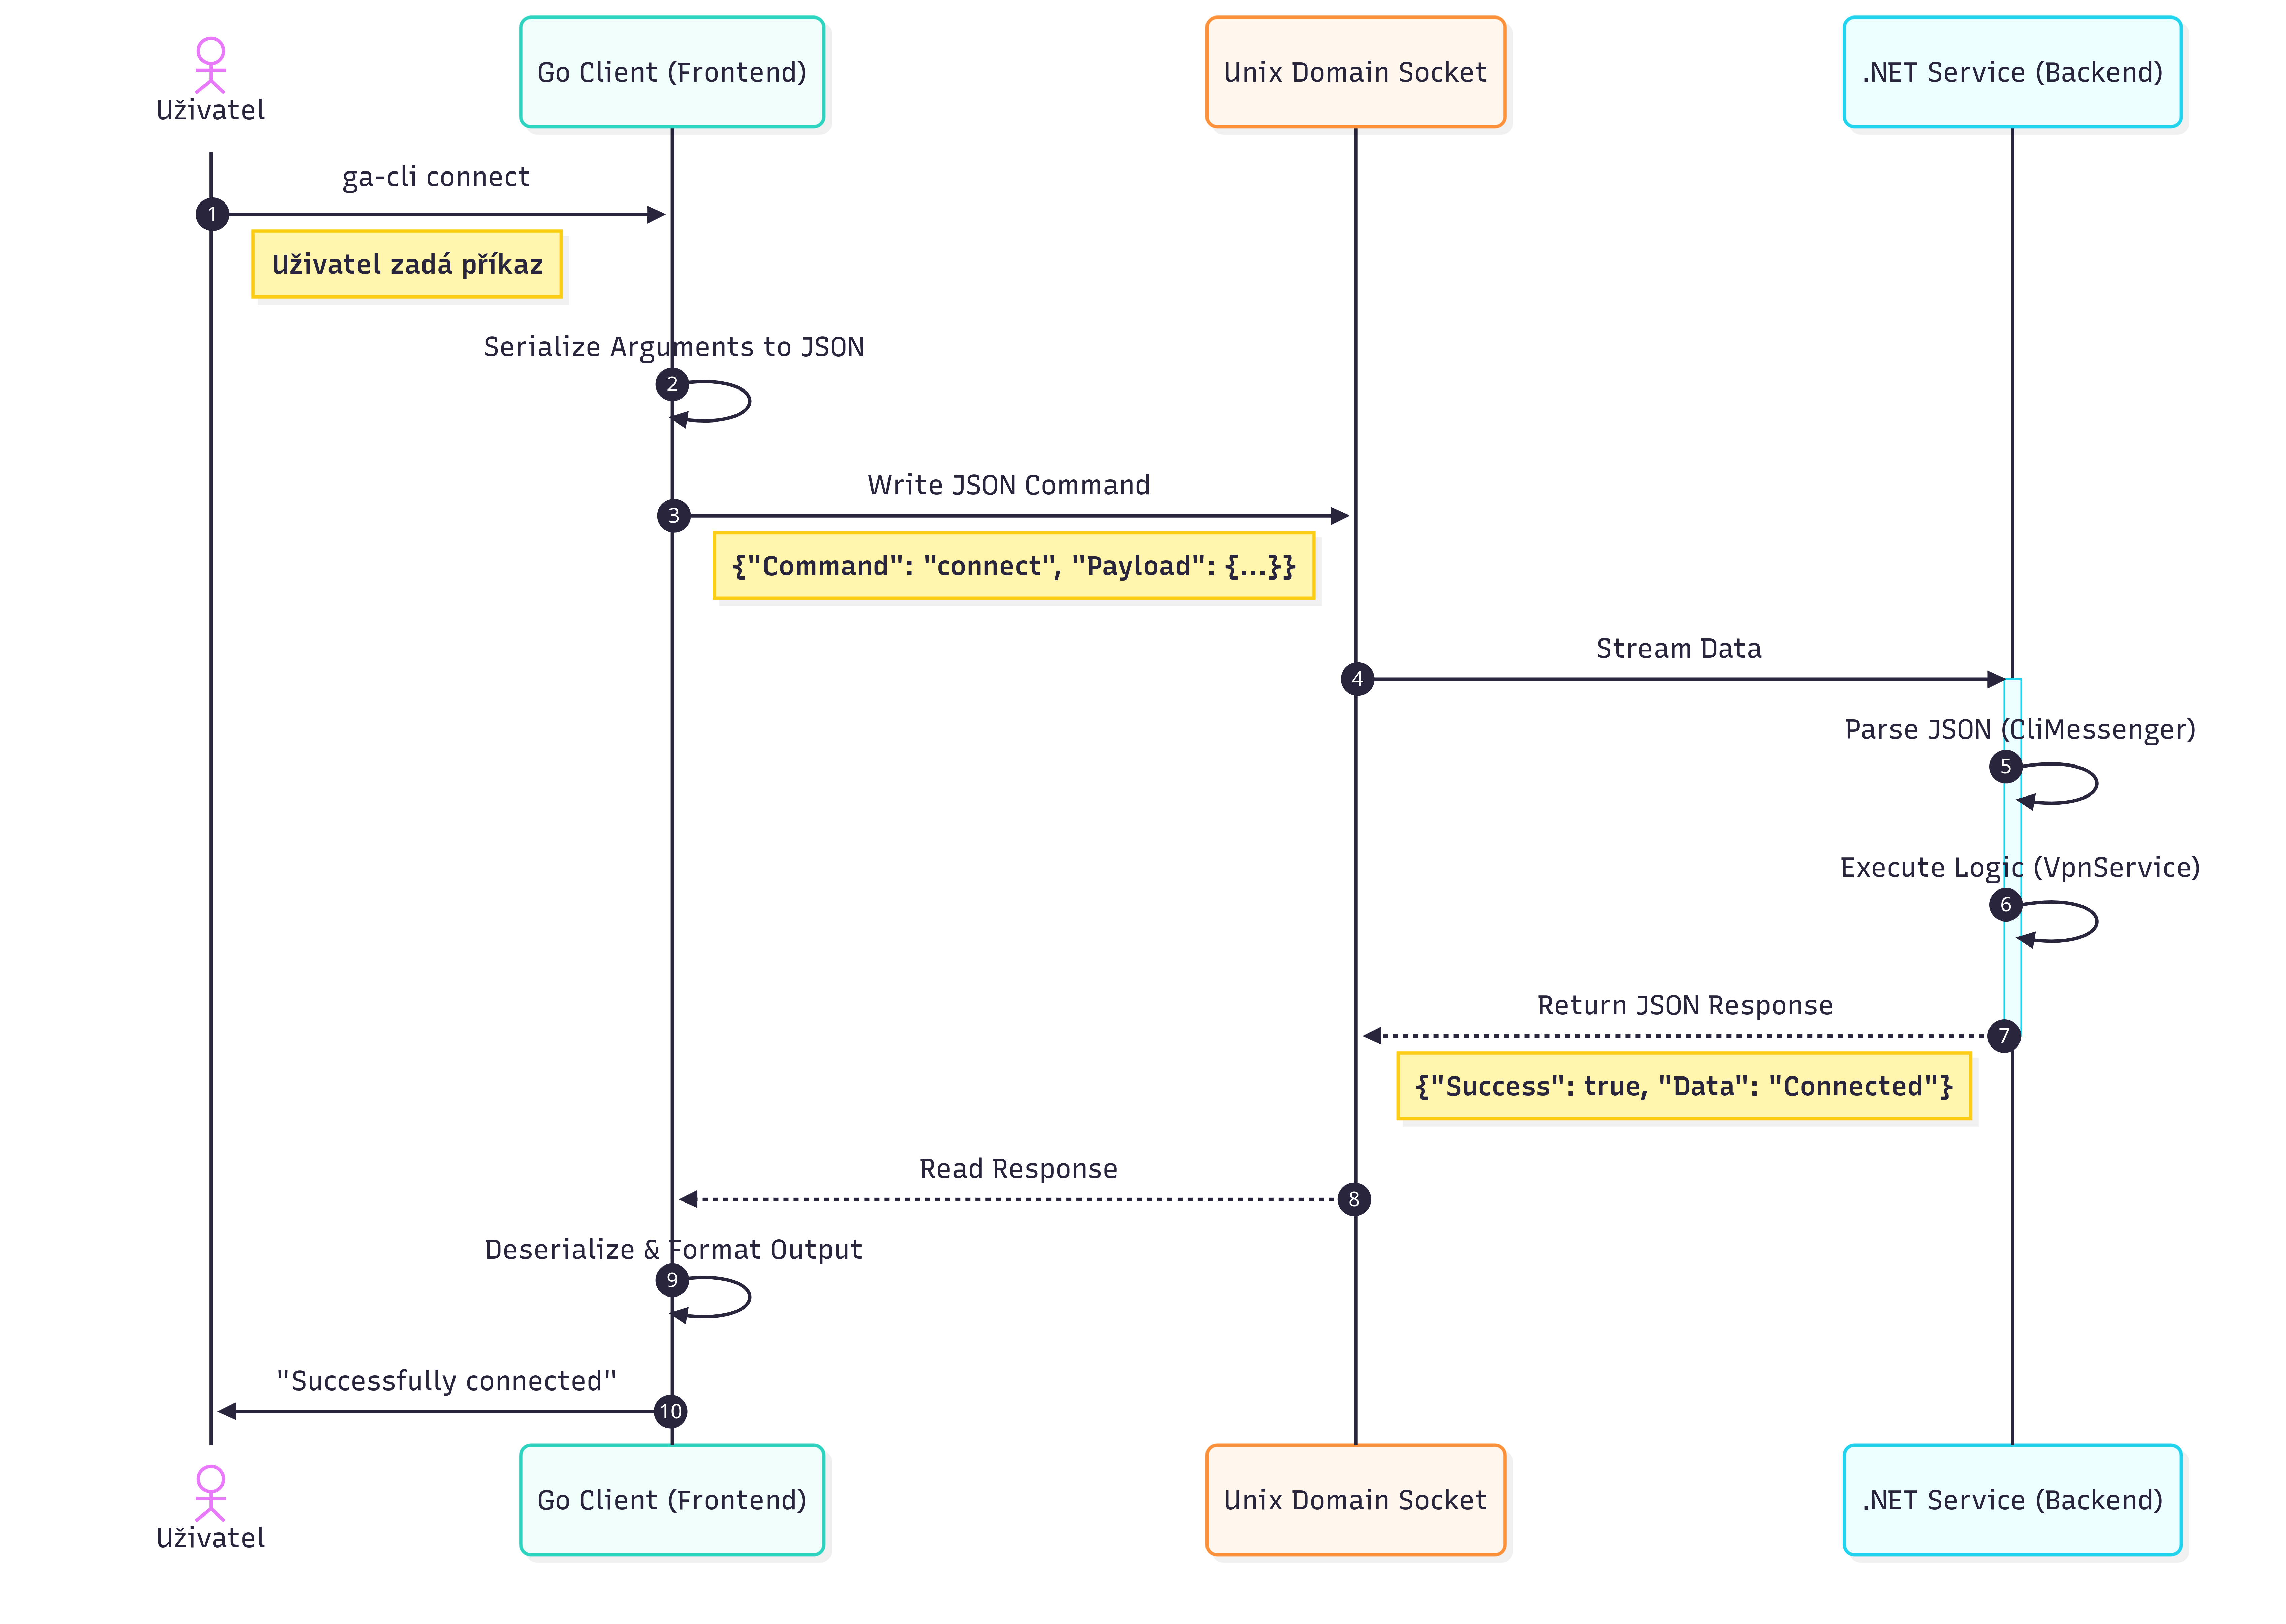
\includegraphics[width=\textwidth, height=0.85\textheight, keepaspectratio]{images/sequence.png}
\end{frame}

% =========================================================================
% SLIDE 7: Ukázka (Live Demo)
% =========================================================================
\begin{frame}{Představení dosažených výsledků}
    \centering
    \Huge \textbf{Live Demo}
    
\end{frame}

% =========================================================================
% SLIDE 8: Harmonogram
% =========================================================================
\begin{frame}{Harmonogram a stav práce}
    \textbf{Hotovo:}
    \begin{itemize}
        \item[\checkmark] Implementace komunikačního rozhraní (IPC).
        \item[\checkmark] Backend logika v .NET.
        \item[\checkmark] Frontend klient v Go.
        \item[\checkmark] TDD testy pro klíčové scénáře.
    \end{itemize}

    \textbf{Probíhá:}
    \begin{itemize}
        \item[\textbf{...}] Refaktorizace a ladění edge-cases (řešení konfliktů).
        \item[\textbf{...}] Psaní textové části práce (teorie).
    \end{itemize}

    \textbf{Plán:}
    \begin{itemize}
        \item[$\rightarrow$] Březen: Testování a finalizace balíčků.
        \item[$\rightarrow$] Duben: Odevzdání bakalářské práce.
    \end{itemize}
\end{frame}

% =========================================================================
% SLIDE 9: Závěr
% =========================================================================
\begin{frame}
    \centering
    \Huge \textbf{Děkuji za pozornost}
    
    \vspace{1.5cm}
    \Large Prostor pro vaše otázky
\end{frame}

\end{document}
